\documentclass[12pt]{article}
\usepackage{url}
\usepackage{graphics}
\usepackage{geometry}
\usepackage[table,xcdraw]{xcolor}
\usepackage{tikz}
\usepackage{pgfplots}
\usepackage{pgf}
\usetikzlibrary{shapes,arrows,backgrounds,fit}
\usepackage{longtable}
\usepackage{setspace}
\usepackage{textcomp}
\usepackage{enumitem}
\usepackage{booktabs}
\usepackage{float}
\usepackage{amsmath}
\usepackage{pdfpages}
\usepackage{amsmath}
\usepackage{mathptmx}
\usepackage{anyfontsize}
\usepackage{t1enc}
\usepackage{adjustbox}
\usepackage{array}
\usepackage{graphicx}
\usepackage{caption}
\usepackage[list=true]{subcaption}
\usepackage[table]{xcolor}
\usepackage{multirow}
\usepackage{array}
\usepackage{placeins}
\usepackage{indentfirst}
\usepackage{sectsty}
\usepackage{tocloft}
\usepackage{chngcntr}


\doublespacing


\counterwithin{figure}{section}
\counterwithin{table}{section}

\pgfplotsset{compat=1.14}



%Penalty for floats (images, tables..) to try and keep them within the chapter the are included in...Doesnt work well, use the float barrier instead, much better
\widowpenalty 10000
\clubpenalty10000

%Margins as defined by URIs formatting
\geometry{margin=1in,lmargin=1.5in,bottom=1in}


%%%%%%%%%%%%%%%%%%%%%%%%%%%%%%%%%%%%%%%%%%%%%%%%%%%%%%%%%%%%%%%%%%%%%%%%%%%%%%%%%%%%%%%%
%                                                                                      %
%                     Sets Various Sections on the Title Page                          %
%                                                                                      %
%%%%%%%%%%%%%%%%%%%%%%%%%%%%%%%%%%%%%%%%%%%%%%%%%%%%%%%%%%%%%%%%%%%%%%%%%%%%%%%%%%%%%%%%
\renewcommand{\cftsecleader}{\cftdotfill{\cftdotsep}}                                  %
\newenvironment{bottompar}{\par\vspace*{\fill}}{\clearpage}                            %
\newenvironment{midpar}{\par\vspace*{\fill}}                                           %
%%%%%%%%%%%%%%%%%%%%%%%%%%%%%%%%%%%%%%%%%%%%%%%%%%%%%%%%%%%%%%%%%%%%%%%%%%%%%%%%%%%%%%%%




%%%%%%%%%%%%%%%%%%%%%%%%%%%%%%%%%%%%%%%%%%%%%%%%%%%%%%%%%%%%%%%%%%%%%%%%%%%%%%%%%%%%%%%%
%                                                                                      %
%                     Sets the font size for subsections titles                        %
%                                                                                      %
%%%%%%%%%%%%%%%%%%%%%%%%%%%%%%%%%%%%%%%%%%%%%%%%%%%%%%%%%%%%%%%%%%%%%%%%%%%%%%%%%%%%%%%%
\sectionfont{\fontsize{12}{12}\selectfont}                                             %
\subsectionfont{\fontsize{12}{12}\selectfont}                                          %
\subsubsectionfont{\fontsize{12}{12}\selectfont}                                       %
%%%%%%%%%%%%%%%%%%%%%%%%%%%%%%%%%%%%%%%%%%%%%%%%%%%%%%%%%%%%%%%%%%%%%%%%%%%%%%%%%%%%%%%%



%%%%%%%%%%%%%%%%%%%%%%%%%%%%%%%%%%%%%%%%%%%%%%%%%%%%%%%%%%%%%%%%%%%%%%%%%%%%%%%%%%%%%%%%
%                                                                                      %
%     create table of contents, list of figures, and list of tables....                %
%                                                                                      %
%%%%%%%%%%%%%%%%%%%%%%%%%%%%%%%%%%%%%%%%%%%%%%%%%%%%%%%%%%%%%%%%%%%%%%%%%%%%%%%%%%%%%%%%
\renewcommand{\contentsname}{\hfill\bfseries\normalsize TABLE OF CONTENTS\hfill}       %
\renewcommand{\listtablename}{\hfill\bfseries\normalsize LIST OF TABLES\hfill}         %
\renewcommand{\listfigurename}{\hfill\bfseries\normalsize LIST OF FIGURES\hfill}       %
\renewcommand{\cftaftertoctitle}{\hfill}                                               %
\renewcommand\refname{BIBLIOGRAPHY}                                                    %
%%%%%%%%%%%%%%%%%%%%%%%%%%%%%%%%%%%%%%%%%%%%%%%%%%%%%%%%%%%%%%%%%%%%%%%%%%%%%%%%%%%%%%%%







%% Citation Controllers %%
\newif\ifpaper
\newif\ifIEEE


%%%%%%%%%%         Choose between Print and Electronic copies            %%%%%%%%%%%%%%%      

%\papertrue   % <-  UnComment for paper Version
%\paperfalse   % <-  UnComment for Electronic Version



%%%%%%%%%% When Switiching Between the two formats be sure to delete all %%%%%%%%%%%%%%%
%%%%%%%%%%             compiled files from the thesis folder             %%%%%%%%%%%%%%%   
                
\IEEEtrue % <- UnComment to use IEEE Citation Format
%\IEEEfalse % <- UnComment to use APA Citation Format 



\ifIEEE
	\usepackage{notoccite}
\else
	\usepackage{apacite}
\fi


\begin{document}

%Call title
\clearpage\thispagestyle{empty}
\begin{center}
	THE NAME OF YOUR THESIS IN CAPS \break
	BY \break	
	YOUR NAME
	\begin{midpar}
		A THESIS SUBMITTED IN PARTIAL FULFILLMENT OF THE \break
		REQUIREMENTS FOR THE DEGREE OF \break 
		MASTER OF SCIENCE \break
		IN \break
		SYSTEMS ENGINEERING \break
	\end{midpar}
	
	\begin{bottompar}
		UNIVERSITY OF RHODE ISLAND \break
		2018
	\end{bottompar}
\end{center}



%Grab pdf files for thesis preamble, for electronic or paper
\ifpaper
	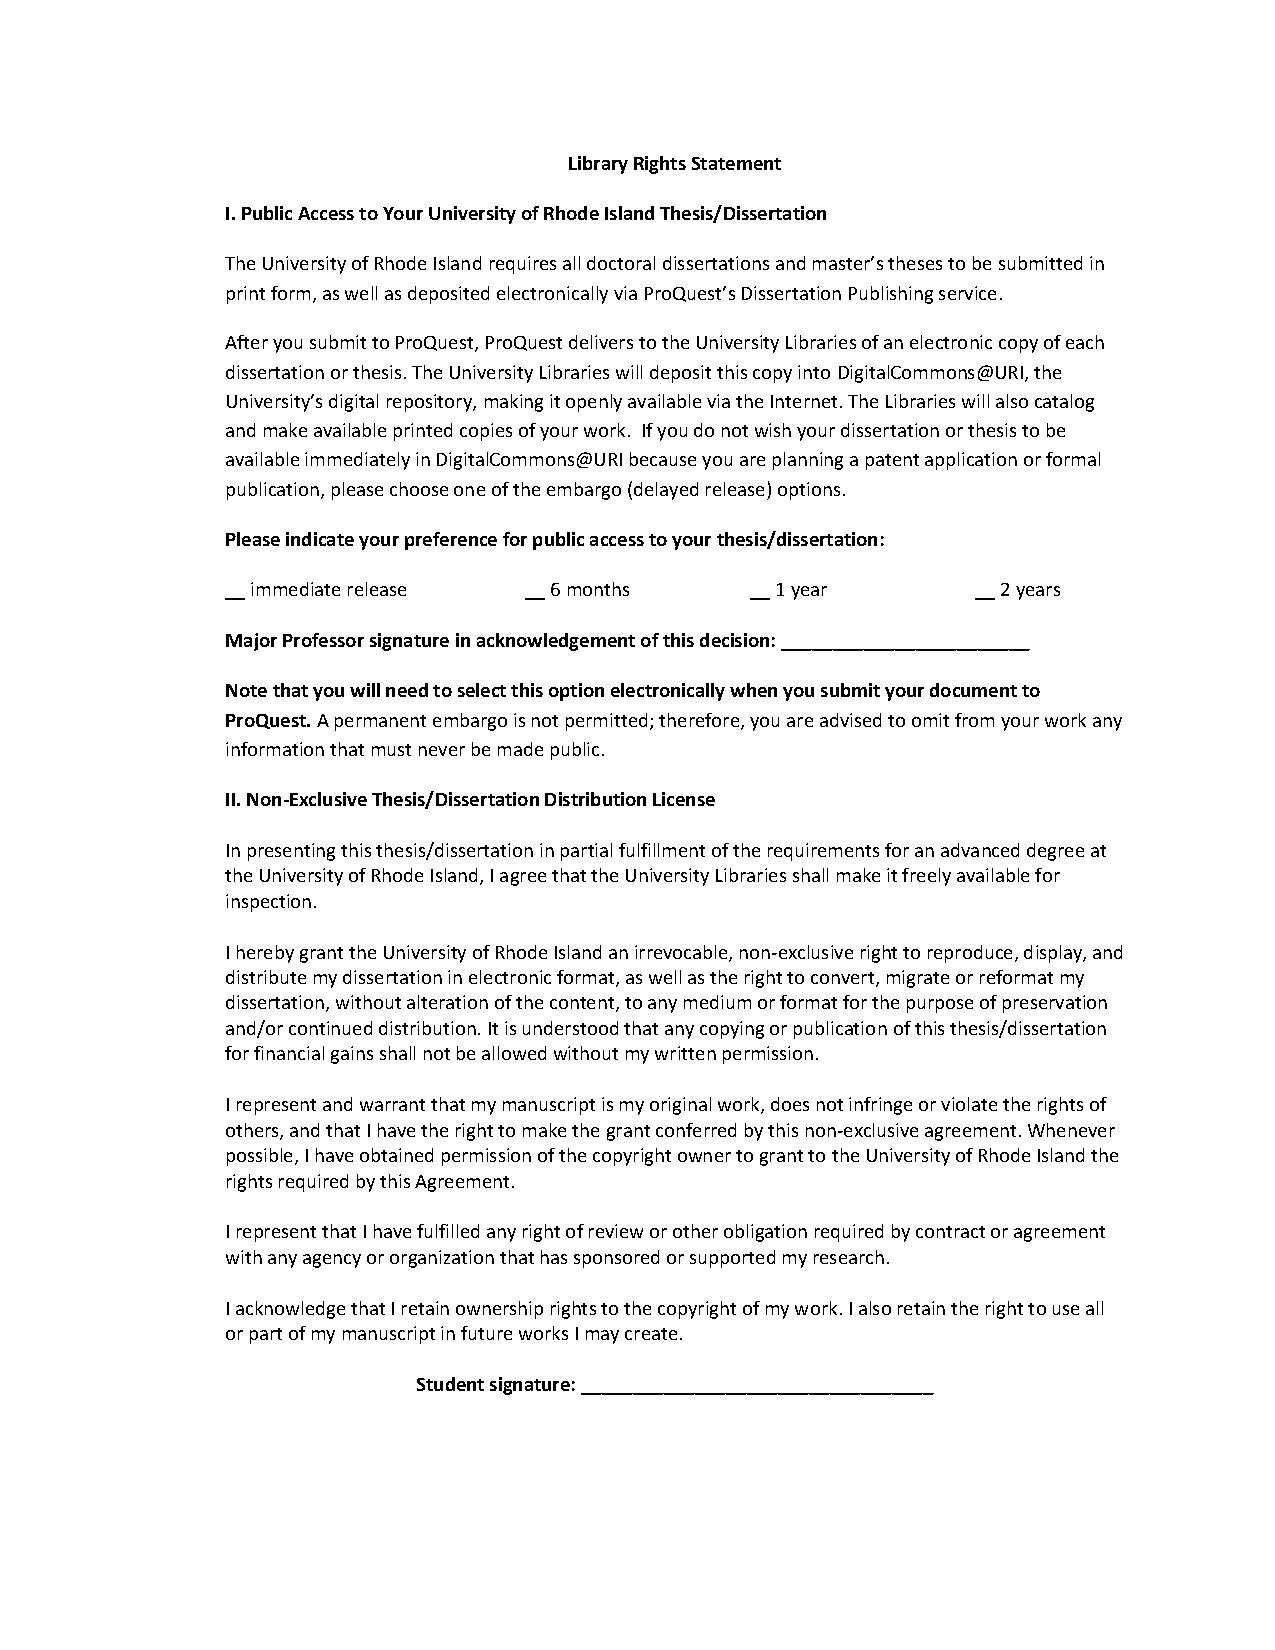
\includepdf[pages=-, offset=0 0]{intropages/library_rights_statement.pdf}
	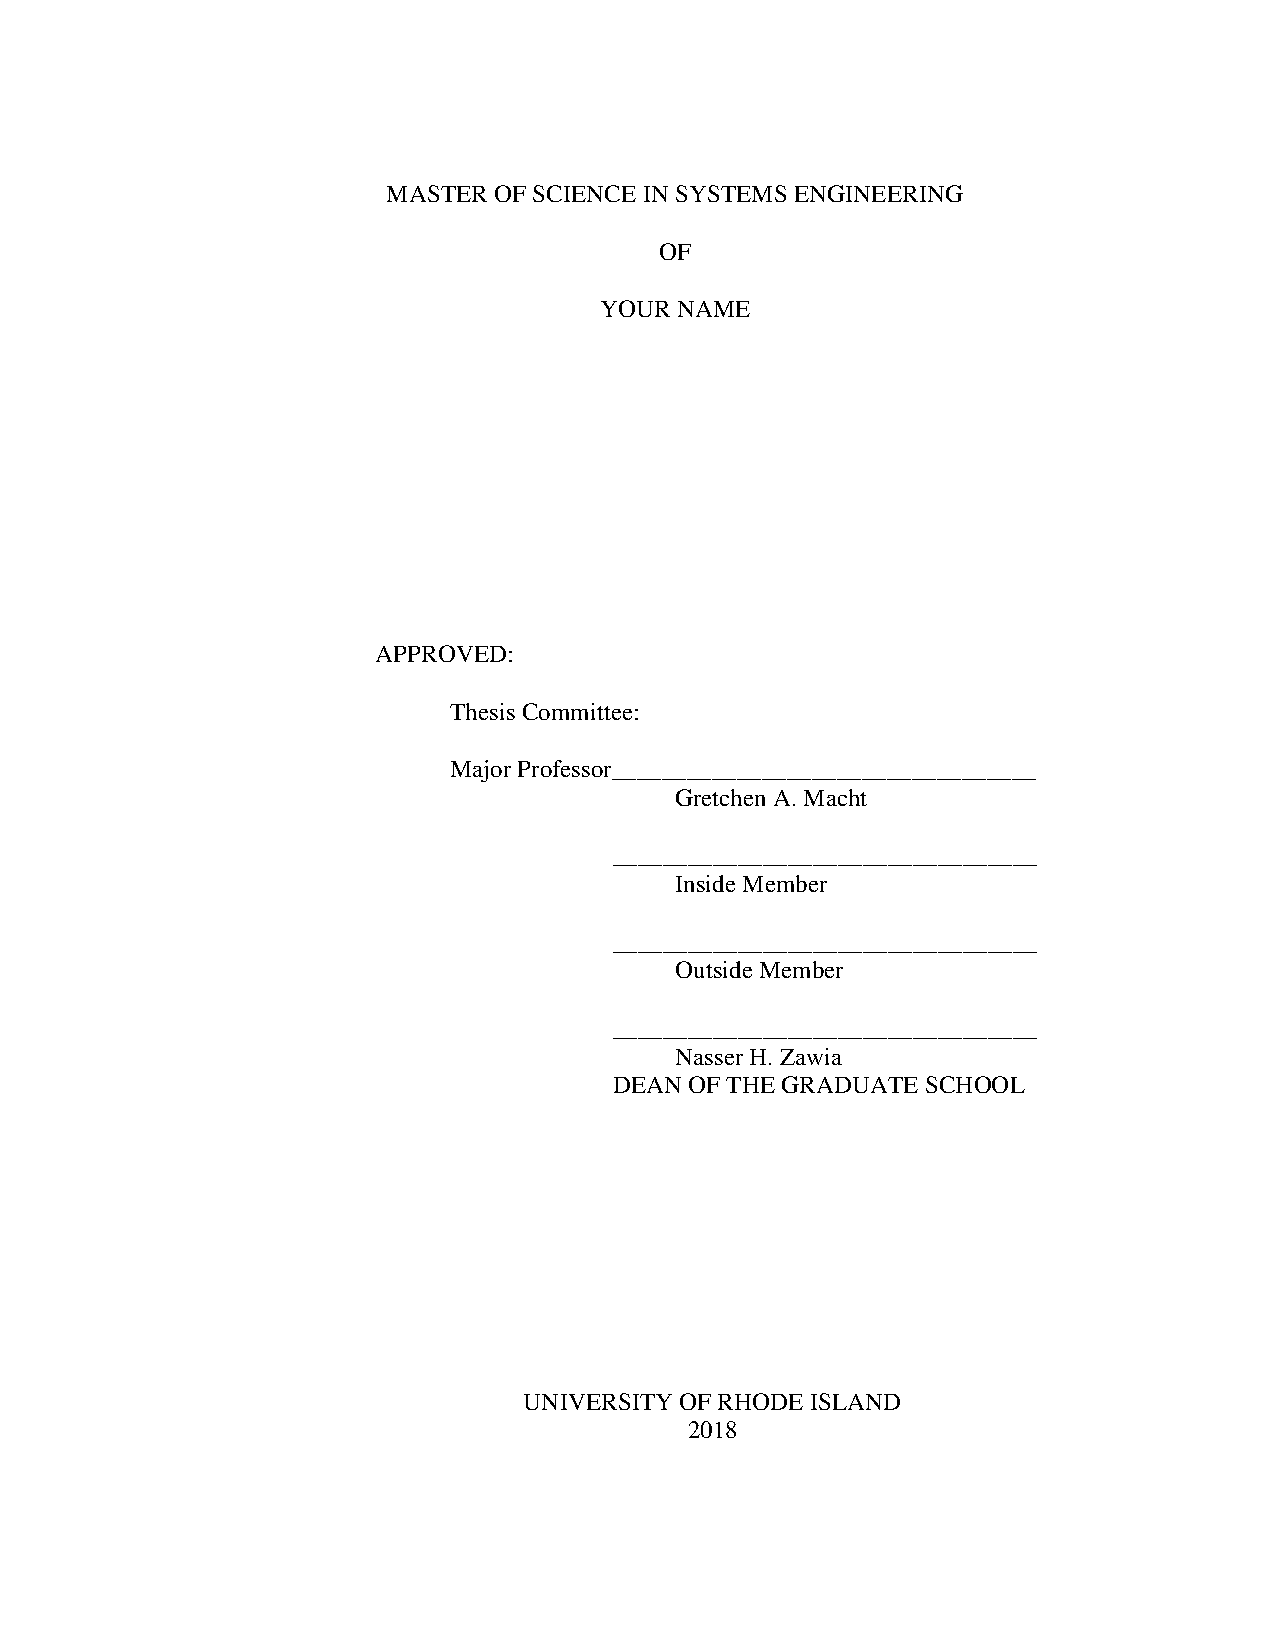
\includepdf[pages=1, offset=0 0]{intropages/sign_pages.pdf}
\else
	\includepdf[pages=2, offset=0 0]{intropages/sign_pages.pdf}
\fi
%-------------------------------------------------------------------------



%Roman numeral numbering until chapter 1
\pagenumbering{roman}

%---------------------- Compile Intro Pages-------------------
\begin{center}
	\section*{ABSTRACT}
\end{center}
\addcontentsline{toc}{section}{ABSTRACT}
\setcounter{page}{2}
%\newpage
\thispagestyle{empty} %< - Add this to every page of the abstract, there are no physical numbers on these pages, but they do exist in the abstract 



\startacknowledgments


Say thanks here if you want....


\tableofcontents
\addcontentsline{toc}{section}{TABLE OF CONTENTS}
\listoftables
\addcontentsline{toc}{section}{LIST OF TABLES}
\listoffigures
\addcontentsline{toc}{section}{LIST OF FIGURES}
\newpage
\begin{center}
	\section*{LIST OF ABBREVIATIONS}
	\setcounter{section}{0}
\end{center}
\addcontentsline{toc}{section}{LIST OF ABBREVIATIONS}
\vspace{5mm}


\begin{longtable}{p{2cm} l}
	ABO & Abbreviation One \\
	ABT & Abbreviation Two\\

\end{longtable}
	
	
	


%-----------------------------------------------------------

\newpage
% Numerical ordring for the rest of the thesis
\pagenumbering{arabic}


%-----------------Compile Chapter Files--------------------

%%%%%%%%%%%%%%%%%%%%%%%%%%%%% Preamble %%%%%%%%%%%%%%%%%%%%%%%%%%%%%%%%%%
\begin{center}                                                          %
	\section*{CHAPTER 1}
	\textbf{Name of Chapter 1}                            %
	\setcounter{section}{1}                                             %
	\setcounter{table}{0}                                               %
	\setcounter{figure}{0}                                              %
\end{center}                                                            %
\addcontentsline{toc}{section}{CHAPTER 1 - Name of Chapter 1}           %
\vspace{5mm}                                                            %
%%%%%%%%%%%%%%%%%%%%%%%%%%%%%%%%%%%%%%%%%%%%%%%%%%%%%%%%%%%%%%%%%%%%%%%%%

The Current Setup supports a 5 chapter thesis. To add additional chapters, create a new chapter folder, with a new tex file. Copy and past the preamble above into the new chapters tex file. Update the \\setcounter{number}, to the chapter number. Change both \\section*{} and the \\addcontentsline{toc}{section}{CHANGE} command to the name of the new chapter. Add the chapter in the thesismain.tex file as well.


\cite{IndustEclog}

\subsection{This Is a Chapters Section} %Create Sections within a chapter

%Images can be saved in individual chapter folders and called like this
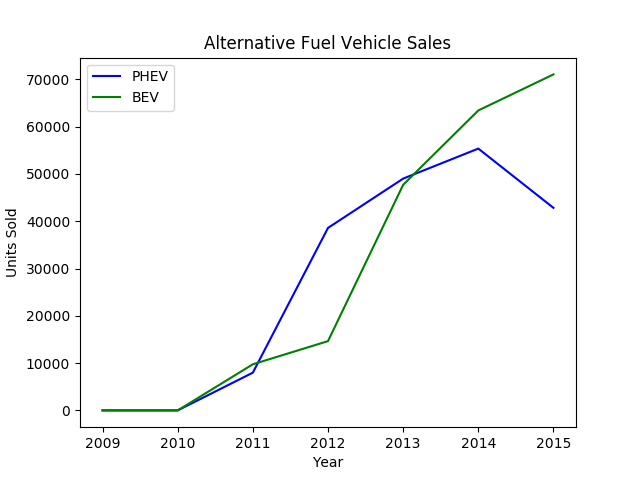
\includegraphics[width=\linewidth]{chapter1/sales}


\subsubsection{This Is a Subsection in a Chapter} %Create a Subsection





  





\begin{center}
	\singlespacing
	\section*{CHAPTER 2}
	\textbf{Name of Chapter 2}
	\setcounter{section}{2}
	\setcounter{subsection}{0}
	\setcounter{table}{0}
	\setcounter{figure}{0}
\end{center}
\addcontentsline{toc}{section}{CHAPTER 2 - Name of Chapter 2}
\vspace{5mm}
\doublespacing






\NewChapter{3}{Name of Chapter 3}

Beging writing chapter 3 here

















\begin{center}
	\section*{CHAPTER 4}
	\textbf{Name of Chapter 4}
	\setcounter{section}{4}
	\setcounter{subsection}{0}
	\setcounter{table}{0}
	\setcounter{figure}{0}
\end{center}
\addcontentsline{toc}{section}{CHAPTER 4 - Name of Chapter 4}
\vspace{5mm}




\begin{center}
	\section*{CHAPTER 5}
	\textbf{Name of Chapter 5}
	\setcounter{section}{5}
	\setcounter{subsection}{0}
	\setcounter{table}{0}
	\setcounter{figure}{0}
\end{center}
\addcontentsline{toc}{section}{CHAPTER 5 - Name of Chapter 5}
\vspace{5mm}



%---------------------------------------------------------


%---------------------Bib/Appendix------------------------
\Appendix

\section*{Appendix A - Extra Stuff}


\addcontentsline{toc}{section}{BIBLIOGRAPHY}
\ifIEEE
	\bibliographystyle{IEEEtran}
	\bibliography{IEEEabrv,ThesisBib}
\else
	\bibliographystyle{apacite}
	\bibliography{ThesisBib}
\fi

%---------------------------------------------------------

\end{document}

